% setup the document and include packages
\documentclass{article}[12pt]
\usepackage{graphicx}
\usepackage{amsmath}
\usepackage{amssymb}
\usepackage{cancel}
\usepackage{ntheorem}
\usepackage{algorithm2e}
\usepackage{float}
\usepackage{caption}
\usepackage{fancyvrb}
\usepackage[dvipsnames]{xcolor}
\usepackage[section]{placeins}
\usepackage[toc,page]{appendix}
\usepackage{hyperref}
\usepackage{subfig}

%set stuff for syntax highlighting
%\usepackage{fontspec}
%\usepackage{minted}
%\setsansfont{Calibri}
%\setmonofont{Consolas}
\usepackage{hyperref}
\hypersetup{
    colorlinks=true,
    linkcolor=blue,
    filecolor=magenta,      
    urlcolor=cyan,
}
\urlstyle{same}

\makeatletter
\def\BState{\State\hskip-\ALG@thistlm}
\makeatother

% define Continue for algorithms
\SetKw{Continue}{continue}

% redefine QED symbol
\renewcommand{\qedsymbol}{\rule{0.7em}{0.7em}}

\usepackage{mathtools}
\DeclarePairedDelimiter\ceil{\left\lceil}{\right\rceil}
\DeclarePairedDelimiter\floor{\left\lfloor}{\right\rfloor}

% define lemma and result theorem-styled sections
\newtheorem{lemma}{Lemma}[section]
\newtheorem{result}{Result}[section]

% setup paths for images
\graphicspath{ {../scripts/plots/} }

% Don't print the semicolon in algorithms
\DontPrintSemicolon

% define the title that will be used in the report
\title{CS 440 MP4 \\ Section Q4 \\ 4 Credits}
\author{
Christian Howard \\ howard28@illinois.edu
\and
Luke Pitstick \\ pitstck2@illinois.edu
}
\date{} % don't set a date because we don't need this shit


% start the document
\begin{document}
   
   % create the title page 
   \maketitle
   \begin{abstract}
   \end{abstract}
   \newpage
   
   % create table of contents on separate page
   \tableofcontents
   \newpage
   
   % start section covering work on Part 2
   \section{Pong and Q Learning} \label{sec:two}
   \subsection{General Formulation} \label{sec:pongform}
   To formulate Pong such that it can be used in a Q Learning framework, a Markov Decision Process (MDP) needs to be defined that represents Pong. To this end, we can define $\mathcal{S} \in \mathbb{R}^n$ as the continuous state-space representing the Pong environment and then define $\mathcal{A}$ as a set of finitely many actions that can be taken within the environment. 
   
   Next, we need a transition function $T: \mathcal{S} \times \mathcal{A} \rightarrow \mathcal{S}$ that can give us a new state given a previous state and action pair. This function maintains the Markov property in that it only needs the last state and some corresponding action to obtain the next state. Note that $T(\cdot)$ can internally have randomness associated with it such that a given state-action pair need not produce the same output state each time they are operated on by $T(\cdot)$.
   
   Another important thing to define, which may greatly impact the policy learned via Q Learning, is a rewards function $R: \mathcal{S} \rightarrow \mathbb{R}$ that maps a given state into a scalar that decides how good it is to be in that state. This function will have specific definitions depending on the goal for Pong, so these will be defined later.
   
   Lastly, we need a way to discretize the continuous space into features that can be used to represent the Q values for a given state. Let us define $\mathcal{S}_D$ as the discrete state-space of our environment, then we must have some function $D: \mathcal{S} \rightarrow \mathcal{S}_D$ that takes a continuous state and spits out a discrete state. For added convenience, we can define bijective hash functions $h_s: \mathcal{S}_D \rightarrow \mathbb{N}$ and $h_a: \mathcal{A} \rightarrow \mathbb{N}$ to go from discrete states and actions to indices. From there, we define the Q values representation as a matrix $Q \in \mathbb{R}^{|\mathcal{S}_D|} \times \mathbb{R}^{|\mathcal{A}|} $ and use the hashes for the discrete state and action to retrieve a Q value for some state and action pair.
   
   The Q Learning update algorithm itself, in the complete continuous representation, is then based on the following recursive relationship:
   \begin{align}
   Q(s,a) &= (1 - \alpha) Q(s,a) + \alpha \left( R(s) + \gamma \max_{\hat{a}} Q( T(s,a), \hat{a})\right) \label{eq:qlrn}
   \end{align}
   
   where $(s,a)$ are some state-action tuple, $\alpha \in (0,1]$ is the learning rate, and $\gamma \in [0,1]$ is the discount factor. Using a discrete analog to the above equation, we can over experience get a better representation for $Q$ and in turn develop a better policy $\pi(s)$ where it is defined as:
   
   \begin{align}
   \pi(s) &= \arg \max_{a} Q(s,a)
   \end{align}
   
   Now in terms of training, there are a few things that are being done. For exploration, $\epsilon$-greedy is being used. This means for some probability $\epsilon$, the agent will use a random action and otherwise will use the greedy policy $\pi(s)$ given the current values for $Q$. Additionally, $\alpha$ is being computed using the following equation:
   
   \begin{align}
   \alpha(s,a) &= \frac{C}{C + N(s,a)}
   \end{align}
   
   where $C$ is some constant to be tuned, $N(s,a)$ keeps track of how many times the state-action tuple $(s,a)$ has been visited before. The discount factor $\gamma$ and $C$ are tuned either manually or through a Design of Experiments (DOE).
   
   \subsection{General Implementation}
   The software implemented for this part of the assignment was done in C++. The Q Learning encapsulation was designed as a templated class that used some Template Metaprogramming techniques to allow for defining a Markov Decision Process (MDP) class that can used as a template parameter. 
   
   Additionally, the actual learning method for this Q Learning was also templated such that a user can define a function for choosing $\alpha$ as a function of episode number and state-action pairs and can also pass in a callback function for reporting information about the learning process. Inside this training method, the Q Learning algorithm retrieves discrete state indices, gets actions via the $\epsilon$-greedy exploration-exploitation strategy, updates the MDP state by feeding in the chosen action, gets a reward for the MDP state, and then updates the associated $Q$-values using the reward, the original state-action pair, and the new state. Note that some basic statistical information is taken as an episode is played out, such as the total reward for the current episode and then a moving average of the average reward across all the episodes. After training is complete, the $Q$-values learned are safed off into a binary file that can be read in later.
   
   Software was also implemented for playing games, either with a GUI or without one, against any AI players or Human players or with wall barriers on any side of the game environment. This software was developed with the help of the C library Allegro5 which helped with the GUI and event handling when playing with the GUI. A sample screenshot of the GUI, annoted with which agent is which on the screen, is shown in Figure \ref{fig:gui1}.
   
   \begin{figure}[!htb]
   	\centering
   	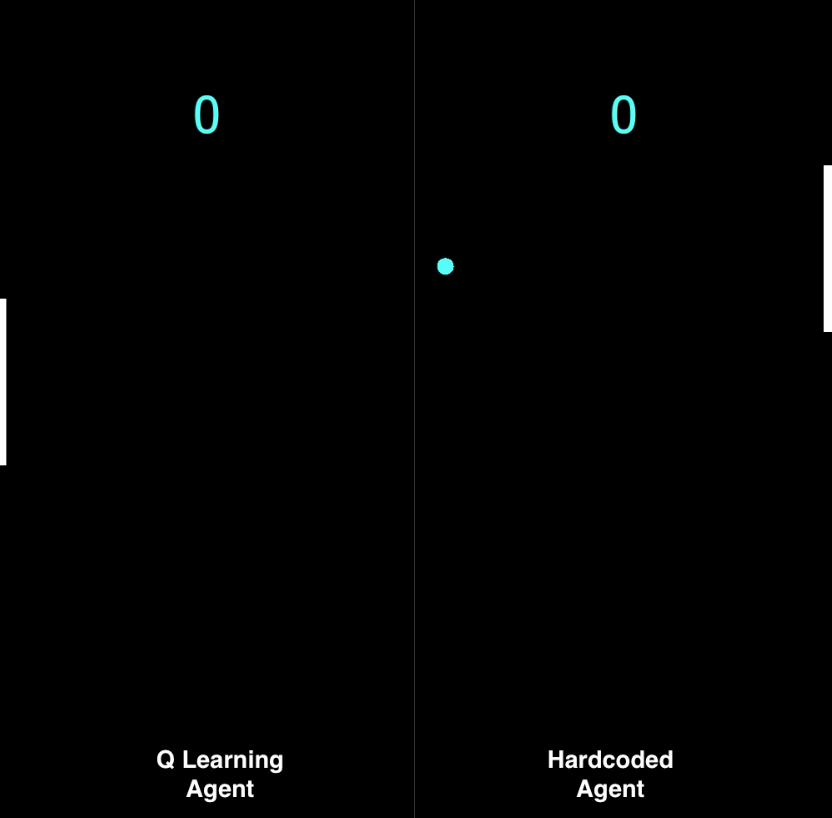
\includegraphics[scale=0.7]{gui_snapshot2.png}
   	\caption{Snapshot of Annotated GUI in middle of Game}
   	\label{fig:gui1}
   \end{figure}
   
   \subsection{Volleying Pong Agent}
   \subsubsection{Formulation}
   For this task, the goal is to come up with a Pong agent via Q Learning that can volley the ball against a wall as long as possible. Let us first define the continuous state as $\mathcal{S} = \left( s_1, s_2, s_3, s_4, s_5\right)$ and the actions set as $\mathcal{A} = \lbrace a_1, a_2, a_3\rbrace $, where the components are defined in Table \ref{tab:vwall}. Note that $h_p$ is the height of the paddle which is set to $h_p = 0.2$ for this problem. The transition function for this problem has the definition found below:
   
   \begin{itemize} 
   	\item The top and bottom of the domain are walls and the ball will bounce off of them without any noise added on top of the reflection
   	\item The left of the domain is a wall as well but a bounce off of this wall can result in random, bounded changes to the velocity dependent on a Uniform distribution
   	\item If the ball gets hit by the paddle on the right side of the domain, the ball will bounce and can have random changes just like those done by the wall
   	\item Ball position vector is otherwise linearly propogated via the ball velocity
   	\item The paddle position is updated directly by the value for an input action $a$
   \end{itemize}
   
    \begin{table}[ht]
   	\centering
   	\begin{tabular}{l | l}
   		\hline
   		Variable & Definition  \\
   		\hline \hline 
   		$s_1 \in [0,1]$ & Ball $x$ position\\
   		$s_2 \in [0,1]$ & Ball $y$ position\\
   		$s_3 \in [-1,1]\setminus (-0.3,0.3)$ & Ball $x$ speed \\
   		$s_4 \in [-1,1]$ & Ball $y$ speed \\
   		$s_5 \in [0, 1-h_p]$ & Paddle top $y$ coordinate\\
   		$a_1 = 0$ & Do not change paddle position\\
   		$a_2 = 0.04$ & Increase paddle position\\
   		$a_3 = -0.04 $ & Decrease paddle position \\
   		\hline
   	\end{tabular}
   	\caption{State and Action variable definitions for Wall Bouncing Pong Agent} \label{tab:vwall}
   \end{table}

	The discrete states $\mathcal{S}_D$ are defined in the following manner, taken directly from the problem statement:
	\begin{itemize} 
		\item Treat the entire board as a $12 \times 12$ grid, and let two states be considered the same if the ball lies within the same cell in this table. Therefore there are 144 possible ball locations.
		\item Discretize the $x$ speed of the ball to have only two possible values, $1$ or $-1$, which represent the sign of the $x$ speed
		\item Discretize the $y$ speed of the ball to have only three possible values: $1$, $0$, or $-1$. It should map to $0$ if $|s_4| < 0.015$
		\item To convert your paddle's location into a discrete value, use the following equation: 
		
		\begin{align*} 
		\text{discrete\_paddle} =  \left\lfloor \frac{12 s_5 }{ 1 - h_p } \right\rfloor
		\end{align*} 
		
		In cases where $s_5 = 1 - h_p$, set $\text{discrete\_paddle} = 11$. As can be seen, this discrete paddle location can take on 12 possible values
		\item Add a special state whenever the ball makes it past the paddle and leaves the game domain, call it $s_e$
	\end{itemize}

	The last thing to do is decide how the rewards are going to be generated. How the rewards function $R(\cdot)$ works is defined below:
	\begin{itemize} 
		\item If the discrete state is special state $s_e$, the reward is $-1$
		\item If the discrete state represents a bounce off of the paddle, the reward is $1$
		\item Otherwise, return reward of $0$
	\end{itemize}

	With these definitions, it is pretty trivial to put together the necessary MDP and state-space information needed to solve Pong using Q Learning. 
   
   \subsubsection{Nominal Results} \label{sec:nrvolley1}
   To create a good agent capable of volleying the ball against a wall in Pong using Q Learning, it was important to come up with choices for $\gamma$, $\epsilon$, and $C$. Choices for $\gamma$, and $C$ were found by doing a small manual Design of Experiments (DOE), specifically a Factorial Experiment. The experiment was based on $\log_{10}(C) \in [0,4]$ and $\gamma \in [0.1, 0.99]$. For $\epsilon$, a function was chosen as the following:
   
   \begin{align*}
   \epsilon(n) &= \frac{k \epsilon_0}{k + n}
   \end{align*}
   
   where $n$ represents the episode number in the training, $k$ is some constant that was chosen as $k = 10^3$, and $\epsilon_0$ is a new tuning parameter. This parameter was experimented with values $\log_{10}(\epsilon_0) \in [-2,0]$. Through experiments with the DOE, it was found that choices for $\gamma$ and $\epsilon_0$ certainly affected convergence to a good policy but that the choice for $C$ was surprisingly vital in getting a good policy quickly. Through experimenting, it was found $\gamma \geq 0.7$, $\log_{10}(C) \geq 3$, and $\epsilon_0 \geq 0.5$ tended to generate quicker convergence to strong policies.  
   
   To obtaining a policy that performed sufficiently well for this volleying Pong agent, the tuning parameters were chosen as $\gamma = 0.75$, $C = 10^4$, and $\epsilon_0 = 0.99$ and the training was over $10^6$ volleying games. After running this volleying Pong agent across $10^5$ games to test its performance, the average number of times per game that the ball bounced off the agent's paddle before the ball escaped past the paddle was $14.43$ bounces per game.
   
   \subsubsection{Results after MDP Modification}
   To see if improved performance could be obtained, the MDP and discrete state representation were slightly modified. First, the rewards were modified such that the agent received a reward of $1$ for bouncing the ball and received a reward of $-10$, instead of the original value of $-1$, if the ball made it past them. The idea to do this is that the agent may discover a bad action quicker with such a heavy penalty. 
   
   Additionally, the $y$ ball position was discretized to have 24 discrete values instead of 12. The reason only the $y$ ball position was refined, instead of both the $x$ and $y$ ball position values, was because the paddle's decision of where to be is more dependent on the ball's $y$ position than the $x$ position. This theory stems from the fact that given the paddle is lined up vertically with the ball, the paddle really only needs to move of the ball has a nonzero $y$ velocity, so it could be useful to keep track of the ball's $y$ position more accurately than the $x$ position.
   
   One should note the training time was really no different since the number of training episodes were set, but the $Q$-values table was twice as large after the above change. After doing the training using the same tuning parameter values and number of episodes for the optimal case described in Section \ref{sec:nrvolley1}, the average number of bounces per game for this new Q Learning agent was found to be 15.07 bounces per game. While not some enormous improvement on the baseline performance of 14.43 bounces per game, it does show some improvement.
   
   
   \subsection{Dualing Pong Agents}
   \subsubsection{Formulation}
   Within this task, the goal was to come up with a Pong agent that could beat another Pong agent hardcoded to essentially track the vertical position of the ball at all times but move with a velocity half that of the Pong agent being trained. To do this, the new Pong agent had a slightly modified state and set of rewards.
   
   For the state, an added state component $s_6$ was thrown in such that $s_6$ represents the opponent paddle's top $y$ coordinate. This continuous state was then discretized in the same manner $s_5$ was. Additionally, a second special discrete state was added for when the ball moves past the opponent's paddle. It should be noted that the added variable $s_6$ multiplies the original state space by the number of discrete values this variable takes, which is a negative since the space requirements are larger, the training time is longer, and chance of touching some discrete state is much less. However, the benefit is that hopefully knowledge of the opponent paddle's position will help the Q Learning agent's paddle perform more strategically.
   
   As for rewards, now a reward of $1$ is given when the ball moves past the opponent's paddle, a reward of $-1$ is given when the ball moves past the Q Learning agent's paddle, and a reward of $0$ is given otherwise. The logic behind this choice is that the agent should only view getting a ball past their opponent as a job well done while having a ball get past them is obviously from doing a poor job. It is expected that this reward system will also require $\gamma$ to be on the larger side so the agent can maintain the value of some move that might take a little bit to see how useful it was on scoring on the opponent.
   
   \subsubsection{Implementation Modifications}
   Relative to the MDP defined for the Volleying Pong agent, the rewards, state representation, and transition function were slightly modified depending on if the MDP should represent the Volleying Pong agent or the Dualing Pong agent situation. These changes were quite trivial, though, so no major code changes were made here.
   
   \subsubsection{Nominal Results}
   To produce the most optimized Q Learning agent seen in our experiments for the Dualing Pong task, the training was done with $\gamma = 0.8$, $\epsilon_0 = 0.99$, $C = 10^4$, and the number of training episodes were $10^7$. With these training parameters in mind, the win rate of the Q Learning agent against the baseline Pong agent can be found to be 97\%, as noted in Table \ref{tab:p22}. 
   
    \begin{table}[ht]
   	\centering
   	\begin{tabular}{l | l }
   		\hline
   		Number of Games Played & Win Rate by Q Learning Agent (\%)  \\
   		\hline \hline 
   		10,000 &  97.04 \\
   		\hline
   	\end{tabular}
   	\caption{Win Rate of Q Learning Agent for Dualing Pong Task} \label{tab:p22}
   \end{table}
   
   A video for this Q Learning agent going up against the hardcoded Pong agent can be found \href{https://www.youtube.com/watch?v=FWLAqNOhF6I}{here}. Note that this video just shows the two AI playing to 50 points.
   
   \subsubsection{Results after Human Playing Agent}
   So to really test the quality of the agent, a human player played against this agent. This test was actually quite interesting because some flaws in the agent's play style became quite apparent. First, it seemed this agent's strategy banked too much on the fact its opponent was going to actively track the vertical position of the ball. Since the human player generally didn't perfectly track the vertical position of the ball as a strategy, sometimes the Q Learning agent would get stumped about what action to take and even stop moving much!
   
   This flaw seemed to be related to the Q Learning agent ending up in a state it had not either seen before or had not seen often enough to get a good idea what action to take while in it. So while the agent performed fairly well, it was not generally good enough to win against the human player when playing the game to a higher number of points.
  
  \subsubsection{Results} \label{sssec:disres}
  For the results generated, we are looking at features with dimension pairs (2,2), (2,4), (4,2), and (4,4). With this set of disjoint block feature dimensions, Table \ref{tab:dis} includes the accuracy and training run-time for each pair, including (1,1) which represents the data collected in Section \ref{ssec:spf}.
  
  \begin{table}[ht]
  	\centering
  	\begin{tabular}{l | l | l | l}
  		\hline
  		Feature Dimension Pair & Training Run-time & Testing Run-time & Accuracy  \\
  		\hline \hline 
  		(1, 1) & 0.155s & 18.08s &77.1\% \\
  		(2, 2) & 0.194s & 4.082s &84.3\% \\
  		(2, 4) & 1.609s & 2.156s &82.7\% \\
  		(4, 2) & 1.734s & 2.036s &84.7\% \\
  		(4, 4) & 183.6s & 0.975s &75.3\% \\
  		\hline
  	\end{tabular}
  \caption{Results information for Disjoint Block Features} \label{tab:dis}
  \end{table}
   
   \subsection{Classification of Spoken Digits}
   Within this problem, the goal is to create a classifier that can distinguish between different digits, particularly digits 1 through 5, based on recordings from a set of different speakers. The data given to us is a labeled set of thresholded Mel-frequency Cepstrum Coefficients (MFCCs). The goal is to create a classifier that can achieve greater than 80\% overall classification accuracy. 
   
   \subsubsection{Problem Formulation}
   For practical purposes, the MFCCs we are given are essentially matrices with binary values for each element of the matrices. If we take each matrix, with $n_r = 30$ rows and $n_c = 13$ columns of binary values, we can vectorize this matrix for use in our framework defined in Section \ref{sec:one}. Doing this gives us $V = \lbrace 0, 1 \rbrace $ and $d = n_c n_r$, given the definitions in Section \ref{sec:one}. Note that we also define $\Omega = \lbrace 1, 2, 3, 4, 5 \rbrace$, where each of the labels correspond to the spoken digit we are classifying. Using this formulation, it is straight forward to use our generic algorithms to build and test a classifier for this problem.
   
   \subsubsection{Results}
   After training and testing the classifier based on the spectrogram data, it was found that the classifier correctly classified 85\% of the testing data. The confusion matrix for the results can be found in Figure \ref{fig:cm22}. Based on the confusion matrix, it appears the digits that were toughest to correctly classify were 4 and 5. Particularly, there was a large misclassification error where the classifier interpreted some of the data labeled 4 as a 2. Additionally, noticeably large misclassification errors occurred with 5 where the classifier interpreted some of the data labeled 5 as 1 or 3.
   

\newpage
\section{Contributions}
\begin{itemize}
\item Christian Howard
	\begin{itemize}
	\item Did Q Learning part of assignment
	\end{itemize}
\item Luke Pitstick
\begin{itemize}
	\item Did Digit Classification part of assignment
\end{itemize}
\end{itemize}   
   
   
\newpage
   \section{List of Potential Extra Credit}
   \begin{itemize}
   \item Made a GUI for Pong
   \item Made the GUI capable of allowing up to two human players to play against any of the AI
   \item Video of Q Learning-based Agent vs. Baseline Agent found \href{https://www.youtube.com/watch?v=FWLAqNOhF6I}{here}.
\end{itemize}      
   
   \newpage
\begin{appendices}

   \section{Open Source Software Used}
   \begin{itemize}
   	\item Standard C++14 Libraries
   	\item \href{http://liballeg.org/}{Allegro5} C library for GUI and event handling
   \end{itemize}

\end{appendices}   
   
   
   
\end{document}